% 测试图片
\chapter{测试题}
测试托i按的

This is a document to test my indent reflash


\begin{figure}[htbp]
     \centering
     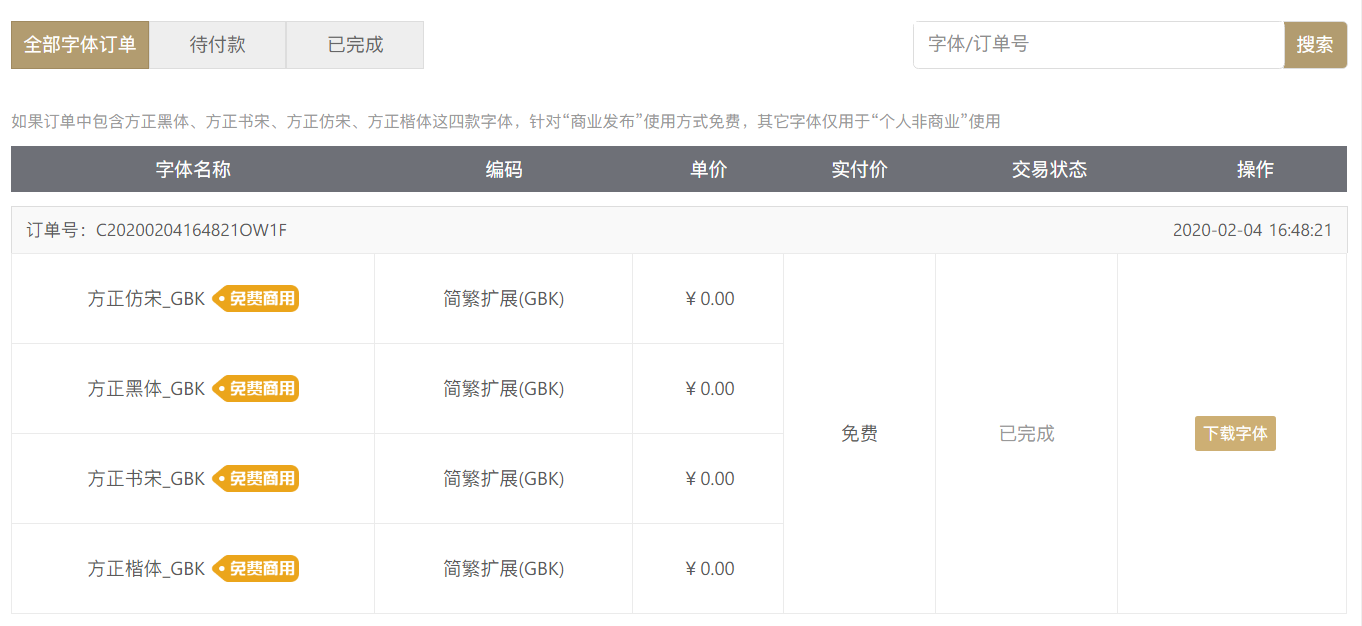
\includegraphics[width = 0.35\textwidth,trim = 10 20 30 40,clip]{founder}
     % \hfill
     \hspace*{2cm}
     % 
\includegraphics[width = 0.35\textwidth,trim = 500 200 300 400,clip,angle=0]{cover16}
     
\includegraphics[width = 0.35\textwidth,angle=0]{cover16}
     \caption{有图有真相}
     \label{fig:myphoto}
\end{figure}

\begin{figure}[htbp]
     \centering
     
\includegraphics[width = 0.35\textwidth]{cover16}
     \caption{有图有真相}
     \label{fig:myphoto}
\end{figure}






     \begin{figure}[htbp]
         \centering
         \begin{minipage}{0.45\textwidth}
             \centering
             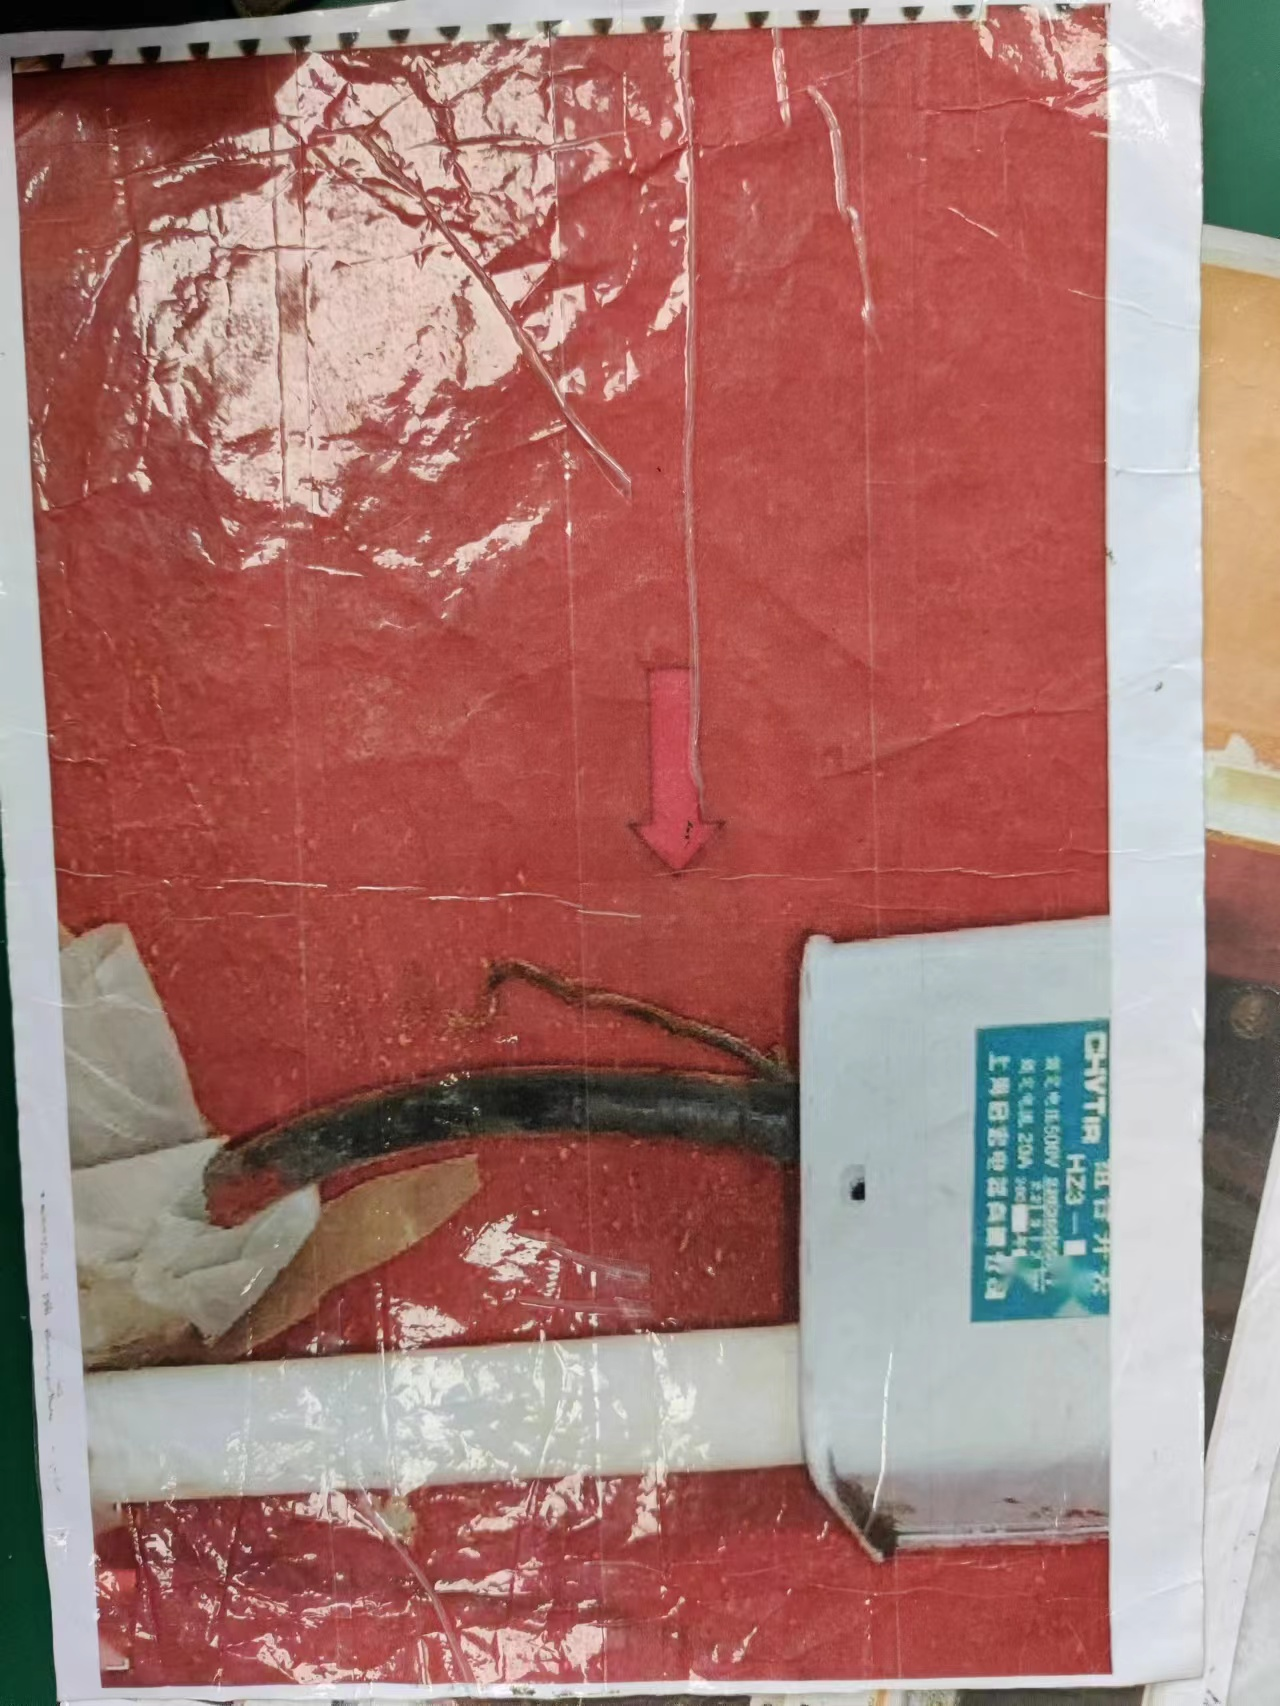
\includegraphics[width=0.9\textwidth]{1}
             \caption{涂鸦}
             \label{fig2}
         \end{minipage}
     %     \hfill
         \begin{minipage}{0.45\textwidth}
             \centering
             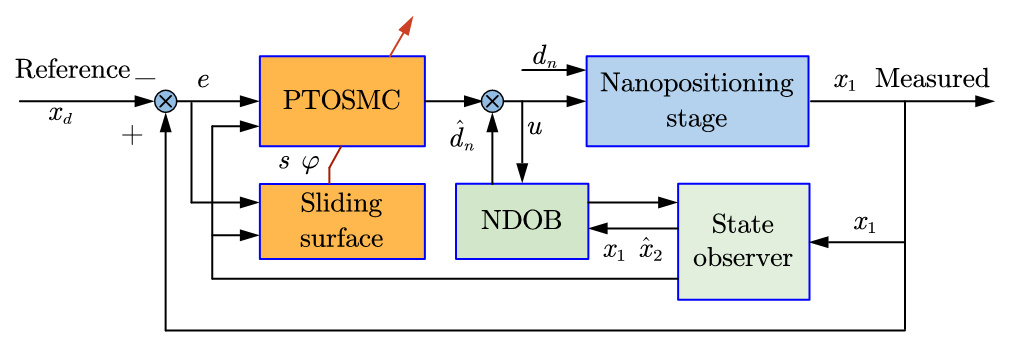
\includegraphics[width=0.9\textwidth]{2}
             \caption{参数为}
             \label{fig3}
         \end{minipage}
     \end{figure}

%%%%%%%%%%%%%%%%%%%%%%%%%%%%%%%%%%%% 表格




     \begin{table}[htbp]
          \renewcommand{\arraystretch}{1.5}
          \centering
          \caption{heading}
          \begin{tabular}{|>{\centering\arraybackslash}p{5cm}|p{3cm}|p{2cm}|}
               \hline
               操作系统& 发行版& 编辑器\\
               \hline
               Windows & MikTeX & TexMakerX \\
               Unix/Linux & teTeX & Kile \\
               macOS & MacTeX & TeXShop \\
               跨平台& TeX Live & TeXworks \\
               \hline
          \end{tabular}
     \end{table}


          \begin{table}
               \renewcommand{\arraystretch}{1.3}
               \centering
               \caption{表格}
               \begin{tabular}{|l|c|>{\centering\arraybackslash}p{2cm}|}
                    \specialrule{0.2em}{0pt}{0pt} % 设置特定行的线宽为0.2em
                    第一列 & 第二列 & 第三列 \\
                    \hline
                    1  &  2 & 6\\
                    \hline
                    5 & 6 &9\\
                    \specialrule{0.2em}{0pt}{0pt} % 设置特定行的线宽为0.2em
               \end{tabular}
               \label{tab1}
          \end{table}

          \begin{table}
               \renewcommand{\arraystretch}{1.3}
               \centering
               \caption{表格}
               \begin{tabular}{lc>{\centering\arraybackslash}p{2cm}}
                    \specialrule{0.1em}{0pt}{0pt} % 设置特定行的线宽为0.2em
                    第一列 & 第二列 & 第三列 \\
                    \hline
                    1  &  2 & 6\\
                    % \hline
                    5 & 6 &9\\
                    \specialrule{0.1em}{0pt}{0pt} % 设置特定行的线宽为0.2em
               \end{tabular}
               \label{tab1}
          \end{table}



          \begin{table}[htbp]
               \centering
             \begin{tabular}{p{80pt}>{\centering}p{80pt}>{\raggedleft\arraybackslash}p{160pt}}
              \toprule
             操作系统& 发行版& 编辑器\\
              \midrule
             Windows & MikTeX & TexMakerX \\
              Unix/Linux & teTeX & Kile \\
             macOS & MacTeX & TeXShop \\
              跨平台& TeX Live & TeXworks \\
             \bottomrule
              \end{tabular}
             \end{table}


%%%%%%%%%%%%%%%%%%%%%%%% 特殊表格
\begin{table}[htbp]
     \centering
     \begin{tabular}{lll}
     \toprule
      & \multicolumn{2}{c}{常用工具} \\
      \cmidrule{2-3}
     操作系统& 发行版& 编辑器\\
      \midrule
     Windows & MikTeX & TexMakerX \\
      Unix/Linux & teTeX & Kile \\
     macOS & MacTeX & TeXShop \\
      跨平台& TeX Live & TeXworks \\
     \bottomrule
     \end{tabular}
\end{table}



\begin{table}
     \centering
     \caption{这是我的表格}
     \renewcommand{\arraystretch}{1.5}
     \begin{tabular}{|c|c|c|c|}
          \specialrule{0.1em}{0pt}{0pt}
          \multirow{2}{*}{内容} & \multicolumn{3}{c|}{标题} \\
          \cline{2-4}
          &苹果 & 相机  & 西瓜\\
          \hline
          重量  & 2 $\mathrm{kg}$ & 3 $\mathrm{kg}$ & 4  $\mathrm{kg}$\\
          体积 & 3 &5&8\\
          面积 & 5 &5 &5\\
          \hline  
     \end{tabular}
\end{table}




\begin{table}[htbp]
      \centering
     \begin{tabular}{P{3.5}P{3.5}}
      \toprule
     \multicolumn{1}{c}{数学常数} &
      \multicolumn{1}{c}{物理常数} \\
     \midrule
     83.14159 & 2.99792 \\
     27.18281 & -17.58819 \\
     3.15123 & 56.48848\\
     22.33333& 62.5265\\
      \bottomrule
     \end{tabular}
      \end{table}

      \begin{table}[htbp]
          \centering
          \begin{tabular}{S[table-format=3.5]S[table-format=2.5]}
              \toprule
              \multicolumn{1}{c}{数学常数} &
              \multicolumn{1}{c}{物理常数} \\
              \midrule
              83.14159 & 2.99792 \\
              27.18281 & -17.58819 \\
              3.15123 & 56.48848 \\
              22.33333 & 62.52650 \\
              \bottomrule
          \end{tabular}
      \end{table}

%%%%%%%%%%%%%%%%%%%%%%% 公式
\begin{equation}
     \begin{array}{c}
         x^2 + y^2 = 2 \\
         y^2 + y^2 = 3 \\
         x^2 + y^2 = 4 \\       
     \end{array}
 \end{equation}

 \begin{equation}
     \begin{split}
         x^2 + y^2 = 2 \\
         \lim_{x \to \infty}  \sum_{i = 1}^n  \frac{1}{2}\\
         xs^2 + \omega y^2 = 2\\
     \end{split}
 \end{equation}

 \begin{gather}
     x^2 + y^2 = 2    \nonumber\\ 
     \lim_{x \to \infty}  \sum_{i = 1}^n  \frac{1}{2}\\
     defe  \nonumber \\
     a+b+c = 4  \nonumber
 \end{gather}

 使用boldsymbol加粗公式,使用displaystyle 完全显示公式,在行内或者array内的公式会被压缩:
        \begin{equation}
            \begin{array}{c}
                \displaystyle
                \min\limits_{\boldsymbol{\omega},b,\xi ,M}  \frac{1}{2} {\boldsymbol{\omega}}^T M^{-1} {\boldsymbol{\omega}}+ C \sum_{i = 1}^{n} \xi_i+ ptr(MS_K) \\
                s.t.y_i\left[ {\boldsymbol{\omega}}^T \cdot \Phi (x_i) +b \right]  + \ge 1- \xi_i,i=1,2, \ldots ,N\\
                \xi_i \ge 0\\
                M \succ 0\\
            \end{array}
        \end{equation}




      
